%% This is an example first chapter.  You should put chapter/appendix that you
%% write into a separate file, and add a line \include{yourfilename} to
%% main.tex, where `yourfilename.tex' is the name of the chapter/appendix file.
%% You can process specific files by typing their names in at the 
%% \files=
%% prompt when you run the file main.tex through LaTeX.
\chapter{Evaluation}

G.E.R.T is a Go-based, bare metal toolkit for embedded applications.
With G.E.R.T, the programmer should be able to implement concurrent embedded programs
which are as performant as the equivalent C implementation, but without having to
worry about concurency abstractions. In order to evaluate G.E.R.T, there are two questions
that must be answered:

\begin{enumerate}
  \item Does G.E.R.T retain good performance despite the costly abstractions of Go?
  \item Do the concurrency patterns of Go simplify the task of the programmer?
\end{enumerate}

The first question is addressed by benchmarks below which measure G.E.R.T's
speed in creating and responding to external events. Pin toggle (\ref{sec:pin_toggle})
measures the maximum pin toggle frequency. Interrupt response time (\ref{sec:int_time})
measures the time it takes to respond to an external interrupt. Pulse counting
(\ref{sec:pulse_count}) counts number of pulses at increasing frequencies.

The second question is harder to answer because difficulty is a subjective
measure. I attempt to show that G.E.R.T presents a better framework for
concurrency through two case studies: a robot sensor platform (\ref{sec:robot})
,which runs motors and reads sensors, and a galvo laser projector (\ref{sec:laser})
which traces images onto a surface by rotating mirrors at high speeds.

In all tests, G.E.R.T is run on an i.MX6Quad SOC and all measurements are taken
with a Rigol DS1054Z oscilloscope. When G.E.R.T is compared to Linux, the SOC
runs Debian 8 "Jessie" with hardfloat support. G.E.R.T is also occasionally
compared to a Teensy 3.2 microcontroller running C. The Teensy 3.2 uses a Cortex M4, which is specifically
intended for microcontroller applications, and has good real-time performance. Its event
response times represent a good comparison point for G.E.R.T and Linux. The Teensy platform
has poor concurrency support though because the Cortex M4 is a single core processor
and it only has 64 kilobytes of RAM.


%%G.E.R.T is evaluated in conditions that are representative of embedded workloads.
%%The first few tests are benchmarks which measure G.E.R.T's maximum interrupt
%%frequency and pin toggle rate. The last two tests are each case studies: a robot
%%sensor platform and a scanning-mirror galvanometer laser projector. The test SOC
%%is the Freescale i.MX6Quad. Depending on the test, it is either running assembly,
%%GERT, or Debian 8 "Jessie" with hardfloat support. A Teensy 3.2 is used for comparison
%%on a few of the latency tests because of its Cortex M4 processor. All timing
%%measurements are taken using a Rigol DS1054Z oscilloscope.

\section{Pin Toggle Frequency}\label{sec:pin_toggle}
This test measures the speed at which G.E.R.T can toggle a simple GPIO pin on
the iMX6 Quad SOC. In ARM assembly, this can be implemented in 4 lines, but compilers and 
abstractions can increase the instruction count. Higher pin
toggling frequency indicates less code in the critical path.
Results are shown in figure \ref{fig:toggle}.


\begin{figure} [h]
\begin{center}
  \begin{tabular}{ | l | l |}
    \hline
    Platform & Avg GPIO Toggle Rate \\ \hline
    ASM & 1.65MHz \\ \hline
    G.E.R.T Unlayered & 568KHz \\ \hline
    Linux C & 263KHz \\ \hline
    G.E.R.T & 154KHz \\ \hline
    Linux Go & 127KHz \\
    \hline
  \end{tabular}
\end{center}
  \caption{GPIO Toggle Rates of Different Platforms}  \label{fig:toggle}
\end{figure}

The results show that G.E.R.T does suffer a performance decrease because of
Go's abstraction cost, but it is correctable. Go's abstraction cost is already
evident from the two Linux benchmarks,
what is not clear is exactly why G.E.R.T underperforms user-space Linux C code.
Without all of the syscalls a user-space program must endure, there should have
been a speed increase.

The slowdown is caused by Go's
interfaces. GPIO pins are represented by an interface in the G.E.R.T embedded package.
In order to toggle a single pin with these interfaces requires 47 instructions:
2 function calls, 19 loads, and 11 stores. If the benchmark program does not use the
embedded package, but toggles the GPIO directly with regular functions,
G.E.R.T achieves a significant speedup. This is indicated by the G.E.R.T unlayered
row in figure \ref{fig:toggle}.

%%s expected, assembly is much faster than any of the other platforms. Additionally,
%it is no surprise that GERT outperforms Go running in userspace Linux. It is not obvious
%why GERT is slower than userspace C code though. An inspection of the GERT bytecode
%yields the answer. To toggle a single GPIO pin in GERT, while using the embedded package,
%takes 47 instructions. Of these 47 instructions, 2 are function calls, 19 are loads, and 11
%are stores. This slowdown is a result of the abstractions present in the embedded package because
%it models each GPIO pin as a Go interface, which comes at a cost.
%When the same pin is toggled in GERT by directly manipulating the memory addresses,
%instead of using the embedded library GPIO abstractions, the
%frequency jumps to 500KHz. This measurement is indicated by the G.E.R.T unlayered row
%in figure \ref{fig:toggle}.

\section{Interrupt Response Time}\label{sec:int_time}
This test measures the time it takes G.E.R.T to respond to an external event
with another external event. Specifically, it is the time it takes to produce
a rising edge on a GPIO pin in response to a falling edge on a different GPIO pin.
G.E.R.T and the Teensy detect the event with hardware interrupts
but Linux polls the input pin in a tight loop because the userspace sysfs
driver does not expose interrupt attachment points.
Results are shown below in figure \ref{fig:RT}.

%%In more complicated programs, a polling loop is disasterous because the program
%%can miss events. G.E.R.T allows the programmer to directly interface with the
%%interrupt controller in order to write true interrupt service routines that miss
%%events far less often. To get the same behavior in Linux,
%%the programmer either has to write a kernel module or hope that a better driver
%%will eventually trickle into the kernel.


%%GERT's advantage is due to its exposed interrupt interface. Utilizing interrupts
%%in Linux would have required a kernel module since the sysfs driver provided
%%no way to interface user-level interrupt handlers. GERT's reponse time is more
%%than adequate for non real-time systems and it may even be appropriate for
%%true real-time systems, depending on what the timing deadlines are. For
%%comparison, a Teensy 3.2 is included in the table because the Cortex M4
%%microcontroller that is has is specifically intended for embedded applications. \\


%%The Teensy has the fastest interrupt response time but G.E.R.T isn't far behind.
%%G.E.R.T is meant to run on a powerful multi-core ARMv7a with more than 1 GB of RAM but the
%%Cortex M4 is only single core and has less than 1MB of RAM. It is also
%%programmed in C.

\begin{figure} [h]
\begin{center}
  \begin{tabular}{ | l | l |}
    \hline
    Platform & Event Reponse Time \\ \hline
    Teensy 3.2 & 1$\mu$s \\ \hline
    G.E.R.T & 6.3$\mu$s \\ \hline
    Linux C & 10$\mu$s \\ \hline
    Linux Go & 30$\mu$s \\
    \hline
  \end{tabular}
\end{center}
  \caption{Event Response Times of Different Platforms}  \label{fig:RT}
\end{figure}

The event response times follow the increasing abstraction cost for each system.
The Teensy is very fast because its interrupt controller is vectored and interrupts
do not cause a stack switch. This means that the Teensy can flip a pin within a few cycles
of receiving the interrupt. G.E.R.T is slower because the iMX6 does not have a
vectored interrupt controller, the interrupt stack must be switched, and the
interrupt handler is written in Go. When G.E.R.T gets an interrupt, it must save its
current state, decide which interrupt it received, and execute its Go handler. Despite this
complexity, the iMX6 can execute more instructions in less time because of its very
high clock rate (792MHz vs 96MHz) so it can keep up with the Teensy.


\section{Pulse Counting}\label{sec:pulse_count}
This test measures G.E.R.T's ability to count incoming pulses. Missed pulses
indicate an excessively long interrupt handler that is still executing when the next
pulse arrives. None of the platforms were configured for re-entrant interrupt handlers
so they can all exhibit this issue.
The pulses are provided by a Xilinx Artix 7 FPGA and they are variable in
frequency and count. The Linux benchmarks are run with polling again because the
userspace sysfs driver does not support interrupt attachment.
Results are shown in figure \ref{fig:counter}.


\begin{figure} [h]
\begin{center}
  \begin{tabular}{ | l | l | l | l |}
    \hline
    Platform & Pulse Count & Max Pulse Rate & Missed Pulses \\ \hline
    Teensy 3.2 & 10 & 2.50MHz & 2 \\ \hline
    G.E.R.T & 10 & 161KHz & 1 \\ \hline
    Linux C & 10 & 161KHz & 4 \\ \hline
    Linux Go & 10 & 50KHz & 1 \\
    \hline
  \end{tabular}
\end{center}
  \caption{Pulse Counts of Different Platforms}  \label{fig:counter}
\end{figure}

G.E.R.T and userspace Linux C achieve the same performance in this test.
It is important to re-iterate though that the userspace Linux programs
are running a tight polling loop. If there were more events to poll or more
systems to control, the performance of Linux would collapse. G.E.R.T, on the
other hand, uses hardware interrupts to register events so its performance will not
collapse.

The Teensy registers more pulses than any other platform because of its
compact and efficient architecture. A dissassembly of the Cortex M4 binary
reveals that all instructions are encoded in 16bit ARM Thumb, as opposed to
32bit ARM that armv7A SOCs use. Additionally, the Cortex M4 uses a vectored
interrupt controller so that the entire length of its interrupt service routine
is only 5 instructions and has no conditionals.

\section{Case Study: Robot Sensor Platform} \label{sec:robot}
In order to evaluate G.E.R.T on a realistic workload, I put it on a robot that was
donated to me from MIT's MASLAB competition. Among other things, the robot has two drive
motors with encoders and also several Sharp GP2Y0A21YK infrared distance sensors on its perimeter.
I wrote a program in Go using G.E.R.T to process all of these event sources at the same time
and operate the robot.

\subsection{Overview}
The main body of the program is an event loop which waits for events coming out of an event channel (fig. \ref{fig:event_loop}).
Independent goroutines monitor each sensor and send events into the event channel. There is a
single goroutine that monitors the event channel and manipulates state in a non-blocking manner. The code for the
event loop is shown below.

\begin{figure}[h]
  \begin{center}
\begin{lstlisting}
select {
	case event := <-event_chan:
		fmt.Printf("%v\n", event)
		switch event {
		case "p":
			val := adc.Read(0)
			fmt.Printf("adc reads %v\n", val)
		case "w":
			drive.Forward(0.2)
		case "s":
			drive.Backward(0.2)
		case "a":
			drive.TurnRight(0.2)
		case "d":
			drive.TurnLeft(0.2)
		case " ":
			drive.Stop()
		}
	}
\end{lstlisting}
\end{center}
  \caption{Robot Event Loop} \label{fig:event_loop}
\end{figure}

\clearpage

Golang's higher order functions and closures were also leveraged in order to create a sensor polling helper function
as shown below in fig. \ref{fig:poll_func}. In this paradigm, every sensor gets its own goroutine which sends
data back into a central event loop.

\begin{figure}[h]
\begin{center}
\begin{lstlisting}
type Pollfunc func() interface{}

func Poll(f Pollfunc, period time.Duration,
sink chan interface{}) chan bool {
	kill := make(chan bool)
	go func(kill chan bool) {
		for {
			select {
			case <-kill:
				return
			default:
				if period > 0 {
					time.Sleep(period)
				}
				sink <- f()
			}
		}
	}(kill)
	return kill
}
\end{lstlisting}
\end{center}
  \caption{Higher Order Polling Function} \label{fig:poll_func}
\end{figure}

\clearpage
The GPIO library was also configured to use interrupts in order to count pulses on the encoder (fig. \ref{fig:encoder}).

\begin{figure}[h]
\begin{center}
\begin{lstlisting}
embedded.WB_JP4_10.SetInput()
embedded.WB_JP4_10.EnableIntr(embedded.INTR_FALLING)
embedded.Enable_interrupt(99, 0) //send GPIO1 interrupt to CPU0
.
//go:nosplit
//go:nowritebarrierec
func irq(irqnum uint32) {
	switch irqnum {
...
	case 99:
		inc()
		embedded.ClearIntr(1)
...
	}
}
.
func inc() {
	count += 1
}

\end{lstlisting}
\end{center}
  \caption{Encoder Interrupt} \label{fig:encoder}
\end{figure}


With these powerful set of abstractions, adding events or sensors into the event loop
is very simple because only a Pollfunc() must be implemented. As an added bonus, this
G.E.R.T program is automatically concurrent because the Go and G.E.R.T schedulers will
move idle cpus to any available goroutine. The rest of this case study explains how the sensors
are interfaced with GERT.

\subsection{PWM Motor Control}
The robot has an MDD10A motor speed controller for controlling the two drive motors. This device
expects a pulse-width modulated signal (PWM) on its input pins in order to direct power into the
motors. A PWM signal has a constant period but the signal is a logical "on" for part of the time
and "off" for the rest of the time. The ratio of "on" time vs the period is called the duty cycle.
It is this percentage which the motor controller translates into a speed for the motor.\\

The iMX6Q includes an on-board PWM peripheral which can output several channels of PWM
at a variety of periods and duty cycles. G.E.R.T contains a driver for this in its embedded
package. The PWM peripheral requires no maintenance once it is configured so the cost of outputting
a PWM signal is essentially a few loads and stores every time the user changes the period or duty cycle.

\subsection{Distance Sensor Reading}
The Sharp distance sensor outputs an analog voltage proportional to its distance from the nearest object (fig \ref{fig:curve}).
A Microchip MCP3008 8-channel ADC is used to convert this into a digital signal. The MCP3008 only communicates in clocked
serial (SPI) though, with 24bit data frames. Luckily, the iMX6Q also has an SPI peripheral. Much like the
PWM peripheral, it has multiple channels that can each concurrently send and receive data. The embedded
package also contains a driver for the ECSPI peripheral and it works much the same way the PWM driver - 
requiring no input from the user other than the data to transmit and the length of the expected response.

\begin{figure}[h]
\begin{center}
  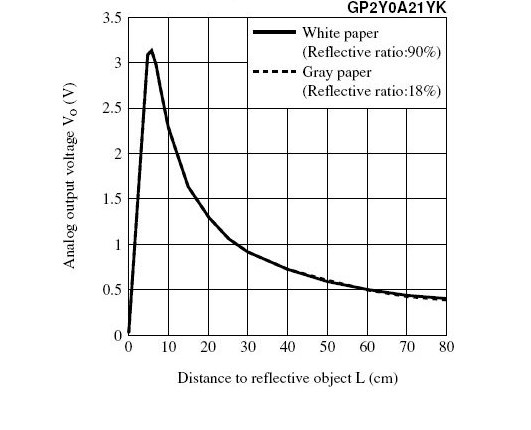
\includegraphics[scale=0.5]{IRSensor-3}
\end{center}
  \caption{Sharp Sensor Distance Curve} \label{fig:curve}
\end{figure}

\clearpage
\subsection{Encoder Reading}
Encoders emit a pulse every time the motor rotates a known amount. This amount is variable depending on the
encoder resolution. The encoders on the test motors emit pulses at a max rate of 4KHz, corresponding to
maximum motor speed. G.E.R.T had no difficulty picking up these pulses because this frequency is far less than
the max pulse frequency in the benchmarks above. A speed monitor was written in fig. \ref{fig:speedmon}
to measure the motor rotation (in Hz) and it corresponded very closely to the oscilliscope readings.

\begin{figure}[h]
\begin{center}
\begin{lstlisting}
//count is updated by the interrupt routine
//and it is the amount of encoder pulses
go func() {
  for {
    old := count
    time.Sleep(1 * time.Second)
    new := count
    event_chan <- new - old
  }
}()
\end{lstlisting}
\end{center}
  \caption{Motor Speed Monitor} \label{fig:speedmon}
\end{figure}

\subsection{Complications}
Systems do not work perfectly, and this robot is no exception. The switching motor controller used
on this robot emits a lot of noise. The 5v noise spikes measured on the oscilloscope wreaked havoc
on the 3.3v single-ended signals that the iMX6 operates with, causing serial communication failures
and spurious interrupts. To deal with this, the motor is operated from a dedicated power supply
when taking encoder measurements. Consequently, the physical robot cannot move when the motors
are connected to an external power supply.

\subsection{Result}
G.E.R.T is a plausible embedded toolkit to use for robots that incorporate many sensor systems.
By utilizing Go's language features, an embedded firmware engineer can implement a complicated sensor integration
platform on top of GERT without worrying about issues like scheduling or shared memory. Go's runtime manages all
of that headache and goroutines also allow for the program to scale with the number of available cpus.


\section{Case Study: Laser Projector}\label{sec:laser}
A scanning-mirror galvanometer laser projector is a device that deflects a laser beam off of several mirrors in
order to draw an image on another surface. If the entire image can be scanned faster than 24Hz, then the light appears
to blend and the human brain perceives it as a single image rather than many points. The maximum rate at which the
projector can trace points is bounded below by the speed of the galvos and bounded above by the speed of the software.
I haven't written the rest of this yet so you will have to use your imagination from here.
